\documentclass[12pt]{article}

\usepackage[T1,T2A]{fontenc}
\usepackage[english]{babel}
\usepackage[type1]{libertine}
\usepackage{microtype}

\babelprovide[import,main]{serbian-cyrillic}

\newcommand\textenglish[1]%
{\foreignlanguage{english}{\fontencoding{T1}\selectfont#1}}
\newenvironment{english}%
{\begin{otherlanguage}{english}\fontencoding{T1}\selectfont}%
	{\end{otherlanguage}}

\NeedsTeXFormat{LaTeX2e}[1994/06/01]
\ProvidesPackage{pek}

\RequirePackage{amsmath, amsfonts, amssymb, amsthm, braket, bbold, fullpage, tikz, pgfplots, pgffor, empheq, mathtools}
\usetikzlibrary {positioning}
\newcommand{\crtNaH}[1]{\draw (#1,-0.1) node[anchor=north] {#1}  [thick] (#1, -0.1) -- (#1, 0.1);}
\newcommand{\bd}{\textbf}
\newcommand{\evl}[3]{|_{#1=#2}^{#1=#3}}


\newcommand{\graf}[7]{
	
	\begin{scope}
		\clip (-0.1,-0.1) rectangle (#1,#3);
		\draw[->] (-0.1,0) -- (#1,0) node[below] {$#2$};
		\draw[->] (0,-0.1) -- (0,#3) node[left] {$#4$};
		
		
		\clip (0,0) rectangle (#1,#3);
		\draw[scale=1,domain=0:#7,smooth,variable=#5,black] plot ({#5}, {#6});
	\end{scope}

	\foreach \n in {1,...,#1}{
		\draw (\n,-0.1) node[anchor=north] {\n}  [thick] (\n-1, -0.1) -- (\n-1, 0.1);
	}

	\foreach \n in {1,...,#3}{
			\draw (-0.1,\n) node[anchor=east] {\n}  [thick] (-0.1, \n-1) -- (0.1, \n-1);
	}
	

	\draw (0,-0.09) node[anchor=north] {0};
}


\endinput
\usepackage{graphicx}
\usepackage{subcaption}
\usepackage{float}
\usepackage[export]{adjustbox}

\usepackage{listings}
\usepackage{color}

\input{listings-glsl.prf}
\lstset{language=GLSL}


\definecolor{dkgreen}{rgb}{0,0.6,0}
\definecolor{gray}{rgb}{0.5,0.5,0.5}
\definecolor{mauve}{rgb}{0.58,0,0.82}

\lstset{frame=tb,
	language=c++,
	aboveskip=3mm,
	belowskip=3mm,
	showstringspaces=false,
	columns=flexible,
	basicstyle={\small\ttfamily},
	numbers=none,
	numberstyle=\tiny\color{gray},
	keywordstyle=\color{blue},
	commentstyle=\color{dkgreen},
	stringstyle=\color{mauve},
	breaklines=true,
	breakatwhitespace=true,
	tabsize=3
}


\title{Рендеровање}
\author{Теодор Ђелић}
\date{Јун 2021}



\begin{document}
	\begin{titlepage}
		\begin{center}
			\vspace*{1cm}
			
			\LARGE
			
			МАТУРСКИ РАД\\
			
			
			\vspace{1cm}
			
			\Huge
			\textbf{Рендеровање}
			
			\vspace{0.5cm}
			
			\LARGE
			Теодор Ђелић
			
			\vspace{1cm}
			
			\Large
			\textbf{Предмет}\\
			\Large
			Примена рачунара\\
			
			\vspace{0.5cm}
			
			\Large
			\textbf{Разред}\\
			\Large
			4-Р\\
			
			\vspace{0.5cm}
			
			\Large
			\textbf{Ментори}\\
			\Large
			Милош Пушић и Филип Радуловић\\
			
			
			\vfill
			
			\vspace{0.8cm}
			
			\large
			
			Прва београдска гимназија\\
			Београд, јун 2021.\\
			
		\end{center}
	\end{titlepage}
	
	\tableofcontents
	
	\pagebreak
	
	\section*{Апстракт}
	У овом раду ћете сазнати шта је компјутерска графика, шта је рендеровање, историјат његовог развоја, као и различите технике његове реализације. Приказаћемо илустрацију рендеровања кроз пример-апликацију која користи модерну имплементацију OpenGL-а.
	
	\section{Увод}
	
	\subsection{Компјутерска графика}
	\paragraph{}
	Компјутерска графика је једна од подобласти компјутерских наука која се, најпростије речено, бави свим процесима који су везани за приказивање слике на екрану, односно од самог процеса обликовања и стварања података који чувају информације облика и модела за приказ, обраде тих информација и текстура, рендеровање и осветљавање модела, све до дигиталних приказа слика на екрану.
	\subsection{Рендеровање као појам}
	\paragraph{}
	Као што смо споменули, рендеровање је кључан део у процесу приказивања слике на екрану. Описали бисмо рендеровање као процес генерисања слике из неких података помоћу софтверског програма. Наравно, овај опис је апстрактан (знамо и сами да се процес генерисања слике у фотошопу разликује од процеса цртања појединачних фрејмова у игрици), па зато и делимо рендеровање по различитим критеријумима на више подгрупа. За критеријум можемо узети разне факторе (нпр. да ли је жељена фотореалистична слика или не), али постоји један који је изнад свих, односно он је онај примарни те га узимамо за главну поделу, а то је критеријум важности брзине извршавања и по њему делимо рендеровање у две категорије: рендеровање у реалном времену и споро рендеровање (тзв. пре-рендеровање). Нпр. у игрици нам је битно да се овај процес одвија јако брзо како би кориснику могли приказати најскорији приказ његовог видокруга како би остварили илузију флуидности, док када бисмо желели да створимо фотореалистичну слику помоћу некакве симулације светлосних зрака, могли бисмо да приуштимо да се тај процес одвија чак и неколико дана, пошто нам је битан само резултат, а не и време за које се тај резултат добије. Но, наравно, ова подела нам и даље не одређује ништа уже процес рендеровања, односно сам процес рендеровања ми дефинишемо и стварамо по томе шта је наш жељени резултат, и ми све те подгрупе називамо различитим техникама рендеровања. Неке од њих ћу споменути и разрадити у каснијем делу рада.
	
	\section{Историјат}
	
	\subsection{Почетак}
	\paragraph{}
	Не постоји боље место одакле бисмо започели причу о историји рендеровања од универзитета у Јути, који са пуним правом можемо назвати колевком компјутерске графике. Једног дана 1965. године, председник универзитета у Јути, Џејмс Флечер, запослио је професора Беркли универзитета, Дејвид Кенон Еванса, да се врати у своји родни град како би основао одсек за компјутерску науку унутар одељења за електронски инжињеринг на универзитету у Јути (овај одсек ће постати засебно одељење 1973). Унајмљени од стране агенције за напредне истраживачке пројекте (на енглескром скраћено ARPA) и финансирани од стране одељења за заштиту Америке, како би могли за њих да развију потребне технологије, подигли су тзв. центар екселенције за компјутерску графику унутар универзитета. Као пионири у развоју компјутерских наука, универзитет у Јути је учествовао у зачетку познатог ARPAnet-а (предак и прототип данашње светске мреже) као један од четири почетна чворишта мреже. Утицај и допринос универзитета на пољу компјутерске графике је толико велики да чак постоји анегдота која каже да скоро свака утицајна особа која припада заједници компјутерске графике је, или прошла кроз универзитет у Јути, или је дошла у контакт са њим на неки други начин.
	
	\paragraph{}
	Било би незахвално када не бисмо споменули неколико имена и њихов допринос на пољу компјутерске графике. Име које се често спомиње уз Дејвида Еванса било би име његовог колеге, Ивана Сатерланда, и они су заједно основали компанију 1968. године која је развијала интерактицне графичке радне станице. Сатерланд је развио апликацију која се узима за претка графичко-корисничког интерфејса под називом Скечпед. Док је сама апликација по себи је могла да производи само најосновније облике, њен значај се одликује у томе што је она била прва, односно, коришћена је као темељ за будуће апликације, које су већ у касним седамдесетим годинама двадесетог века могле да рендерују комплексне објекте. Уз Дени Коена је развио алгоритам (Коен-Сатерландов алгоритам) који се користи за одређивање линија или делова линија које су у видокругу, како би компјутер знао које делове мора да обрађује. Ово је битан зачетни алгоритам у рендеровању, пошто је јако битно (а поготово је тада било битно уз јако ограничавајуће компјутерске компоненте) да се што више смањи број операција које треба да се изврше. Опис и објашњење овог алгоритма је описан у каснијем делу рада (\pageref{koensaterland}. страна). Такође, велики Сатерландов (а тако и Евансов) допринос био је у подучавању студената који су касније итекако допринели развоју компјутерске графике. Један од тих студента био је Гордон Ромни, први студент докторских студија у области компјутерске графике. Неки од његових већих доприноса били су: реалистичне компјутерски генерисане дигиталне слике тродимензионалних виртуалних објеката који су се састојали од планарних троуглова, излазне слике генерисане помоћу растерског скенирања, налик телевизорима тог доба, које су добијане у реалном времену (колико је тадашња технологија то дозвољавала), осветљење и осенчавање објеката помоћу тачкастог светлосног извора, решење за проблем да се цртају само странице које су видљиве из перспективе камере (његов познати пример рендера објекта имена Сома коцка на коме се види да је решен проблем да се цртају само странице које су видљиве, који можете видети на слици са бројем \ref{fig:romni}), алгоритам за сенчење и још неке мање ствари. Морали бисмо споменути још нека имена тог периода, а то су: Алан Ердал - развио је графички интерфејс којим осцилоскоп може да рендерује слике, и такође је у том тренутку реч рендеровање постала део вокабулара компјутерске графике; Едвин Катмул - створио је прву анимацију људске руке и алгоритам (Катмул-Кларков алгоритам) за дељење површине који служи за стварање заобљених површина (\pageref{katmulklark}. страна); Џејмс Блин - програм Пејнт, имплементирао и рефинисао Катмулов алгоритам за рендеровање, бавио се текстурама, рефлекцијама светлости и облим телима (желео је да створи алгоритме који би реалистично рендеровали слике, пример једног рендера можете видети на слици са бројем \ref{fig:blin}). И за крај ове приче о универзитету у Јути којој нема краја, споменуо бих да је најпознатији 3Д модел у свету компјутерске графике, Јутин чајник (слика \ref{fig:jutincajnik}), створен од стране Евановог студента, Мартин Њувела, 1975. године. Овај чајник је заправо био први 3Д модел са заобљеним површинама високог квалитета, те је баш из тог разлога постао познат и коришћен у сврху тестирања програма за рендеровање.
	
	\begin{figure}[H]
		\centering
		\begin{subfigure}[b]{0.4\linewidth}
			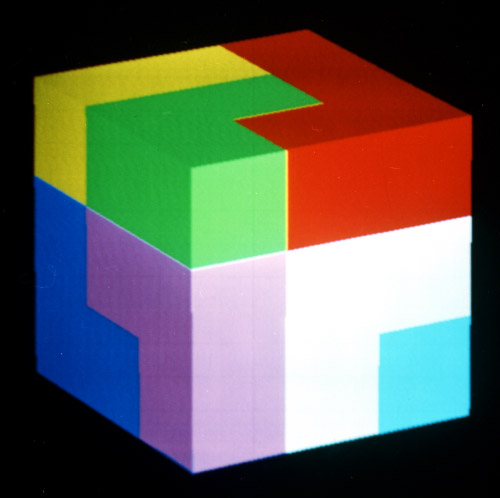
\includegraphics[width=\linewidth]{slike/prviRenderiRomni1.jpg}
			\caption{Рендер склопљене Сома коцке}
		\end{subfigure}
		\begin{subfigure}[b]{0.4\linewidth}
			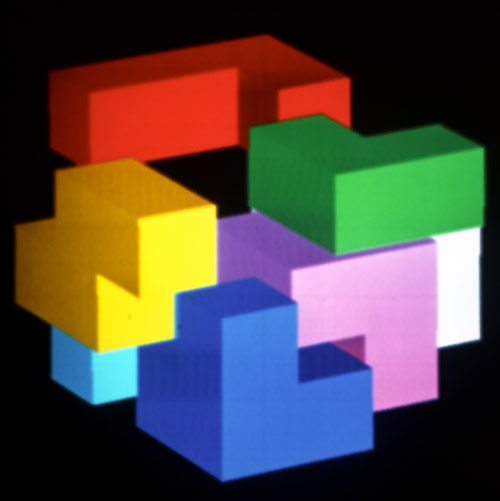
\includegraphics[width=\linewidth]{slike/prviRenderiRomni2.jpg}
			\caption{Рендер раширене Сома коцке}
		\end{subfigure}
		\caption{Рендер Сома коцке}
		\label{fig:romni}
	\end{figure}

	\begin{figure}[H]
		\begin{minipage}{0.4\linewidth}
		\centering
		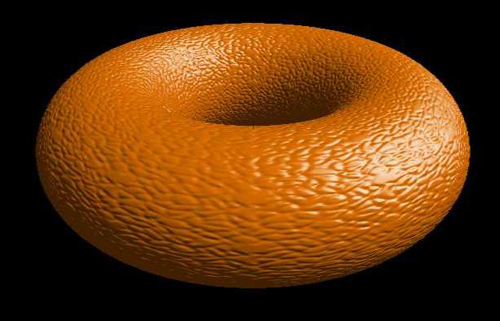
\includegraphics[max width=\linewidth]{slike/prviRenderiBlin.jpg}
		\caption{Блинов рендер облика торуса}
		\label{fig:blin}
		\end{minipage}\hfill
		\begin{minipage}{0.4\linewidth}
		\centering
		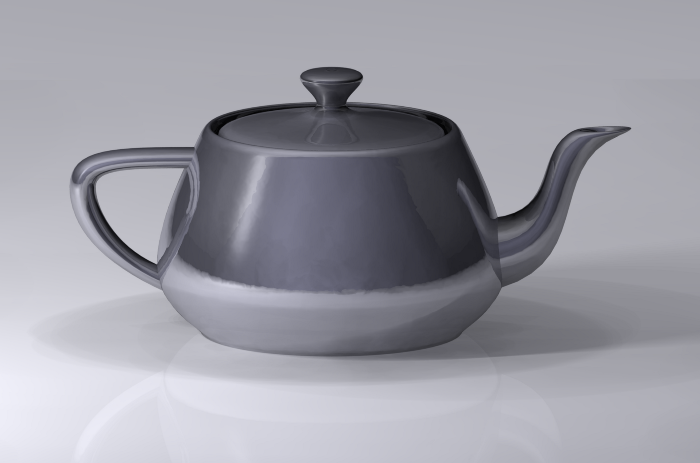
\includegraphics[max width=\linewidth]{slike/jutinCajnik.png}
		\caption{Јутин чајник}
		\label{fig:jutincajnik}
		\end{minipage}
	\end{figure}
	


	\subsection{Развој}
	\paragraph{}
	Временом, како су компјутери постајали јачи и алгоритми све ефикаснији, људи из других области су почели да уочавају вредност, односно начине на које би компјутерска графика могла бити коришћена. Већ средином осамдесетих година двадесетог века, 3Д рендеровани модели су нашли свој значај у архитектури, филмској и музичкој индустрији, а то је био само почетак. Почетком деведесетих година, компанија Пиксар је започела један велики пројекат који ће револуционирати област анимираних филмова. 1995. године, Пиксар је у биоскопима широм света пустио у продукцију филм под називом Прича о играчкама, филм који је у потпуности био 3Д анимиран помоћу компјутера. У ово доба је такође индустрија видео игрица била у процвату, и тада су почеле да се производе игрице које су потпуно биле рендероване са 3Д графиком.
	
	\subsection{Данас}
	\paragraph{}
	Као што верујем да смо сви чули, данас је ударна тема у свеукупној области компјутерских наука машинско учење. Што се тиче компјутерске графике, машинско учење је револуционисало област фотореалистичног рендеровања, и сада се производе слике са толиком тачношћу симулација светлости, и са толиком брзином (у односу на временску тежину феномена који се симулира, а то је транспорт светлости), да када бисте рекли шта је могуће да се рендерује човеку који се њиме бавио пре једно 20-30 година, он би вероватно помислио да су то неке оптичке илузије или варке. Но, најфасцинантније у свему овоме је то што је све ово само почетак, и сваким новим истраживачким радом ове границе се померају све више и више, чак толико да се кроз 2-3 истраживачка рада може постићи нешто што је пре шест месеци звучало немогуће. У каквом фасцинантном добу живимо!
	
	\section{Рендеровање као процес}
	
	\subsection{Увод}
	\paragraph{}
	Желео бих да се присетимо наше псеудо дефиниције рендеровања коју сам изрекао на почетку овог рада, а она гласи да је рендеровање процес генерисања слике из неких података помоћу софтверског програма. Иако је ова дефиниција сама по себи довољна, како бисмо процес рендеровања истински разумели, и како бисмо могли да створимо некакав наш програм, морали бисмо да рендеровање кроз кораке дубље објаснимо.
	\paragraph{}
	Рендеровање бих поделио на следеће кораке: прикупљање података који су нам потребни за рендеровање као нпр. модели, њихове позиције и оријентације на сцени, позиција и оријентација камере која преставља наш видокруг, текстуре, нормалне мапе, итд. (ово је део који није стриктно рендеровање, већ пререквизит за његово одвијање, пошто не бисмо могли да рендерујемо када не бисмо знали шта треба да рендерујемо), затим интерпретирање и процесуирање тих података како бисмо могли да графичкој картици тачно пошаљемо оно што треба да нацрта на екран (ово је срж рендеровања, односно 95\% целог процеса; Све технике рендеровања уствари описују баш овај процес (у целости, или његов део)) ,  и на крају морамо да кажемо графичкој картици на који начин да прочита послате податке, и на који начин да их нацрта. У овом последње описаном кораку, графичкој картици, како бисмо јој рекли како да прочита послате податке и на који начин да их нацрта,  шаљемо програмски код који се зове шејдер (енгл. Shader). Пре него што се упустимо у то како се процесуирају подаци и како се врши комуникација са графичком картицом, ми морамо прво да схватимо и овладамо неким основним структурама података објеката које ћемо сретати при рендеровању.
	
	\subsection{Структуре података објеката}\label{strukturepodatakaproces}
	\paragraph{}
	Било би неефикасно, а такође и непрегледно, када бисмо сваки модел ручно записивали у наш код како бисмо манипулисали њиме. Из тог разлога, људи су смислили да праве засебне фајлове који ће те моделе чувати. Од почетка рада, ми баратамо речју модел без да смо дефинисали шта он тачно представља у компјутеру. Наравно, ми знамо када видимо очима Јутин чајник да је то Јутин чајник, али како је он заправо сачуван. Две најбитније особине модела јесу његова геометрија и његов спољашњи изглед.
	Постоје три различита начина на који се чува геометрија: апроксимирана мрежа, прецизна мрежа и конструктивна геометрија чврстих тела.
	\begin{enumerate}
	\item У случају апроксимиране мреже, модел је заправо сачињен од много малих примитивних облика (полигона) и у ову сврху се најчешће користе троуглови, пошто су они најпримитивнији облик, те могу сачињавати најкомплексније облике (слика \ref{fig:geomTehnika1}). Овај процес где неку површину покушавамо да покријемо облицима који се не секу како бисмо добили тачнију апроксимацију јесте теселација (нпр. у већини програмских језика шејдера постоје шејдери везани за овај процес теселације, и они се користе баш за повећавање резолуције површине односно теселације). У случају коришћења троуглова (троуглови се користе у 99\% формата фајлова који користе апроксимирану мрежу), у фајлу се за сваки троугао чувају његова темена и његов нормални вектор. Нормални вектор представља вектор који почиње у средишту троугла, усмерен је у правцу који је нормалан у односу на површину троугла и његов интензитет је 1 (користи се нпр. како бисмо тачно симулирали како се светлосни зрак одбија од његову површину). Проблем овог начина јесте то што чак иако би довољан број малих троуглова врло добро апроксимирао лопту, он, под број један, никад неће бити истог облика као лопта, а под број два, за јако добру апроксимацију ми бисмо морали да чувамо огроман број троуглова, те би сама величина фајла била велика.
	\item У неким случајевима једноставно не можемо да апроксимирамо мрежу, пошто је она и даље, када бисмо увећали довољно тај модел, пуна равних површина и оштрих ивица. Нпр. при конструисању авиона, једноставно није могуће да се користе апроксимације пошто симулације не би биле исправне. У овом случају, користи се начин под називом прецизна мрежа. Она уместо много троуглова или неких других примитивних облика користи некакве параметарске површи, које могу да се по жељи мењају помоћу параметара који дефинишу ту површину (слика \ref{fig:geomTehnika2}). Чак иако су модели који се стварају овим начином прилично тачни, проблем је то што се јако споро рендерују баш зато што је потребно много времена израчунати сваку тачку која припада том моделу, за разлику од технике апроксимације мреже где већ имамо све тачке. Зато ову врсту фајлова користимо само када морамо, односно је неопходно.
	\item Последња начин је конструктивна геометрија чврстих тела. За разлику од прошла два начина, овај начин уопште не користи мрежу као градивну јединицу, већ ствара моделе тако што сабира или одузима примитивне облике као што су коцке, лопте, ваљци, итд (слика \ref{fig:geomTehnika3}). Са овим начином чувања модела обично раде програми за моделовање у правом свету као нпр. АутоКЕД, пошто се лако модификују модели, и такође се чува сваки корак који је одрађен (пошто нису комплексне операције, већ само сабирање, одузимање и трансформисање примитивних облика). 
	\end{enumerate}
	
	\begin{figure}[H]
		\begin{minipage}{0.4\linewidth}
			\centering
			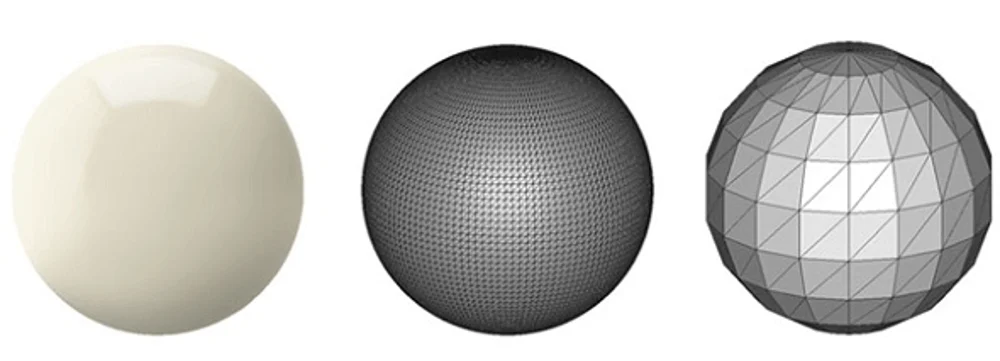
\includegraphics[max width=\linewidth]{slike/strukturePodatakaGeometrijaTehnika1.png}
			\caption{Апроксимирана мрежа}
			\label{fig:geomTehnika1}
		\end{minipage}\hfill
		\begin{minipage}{0.4\linewidth}
			\centering
			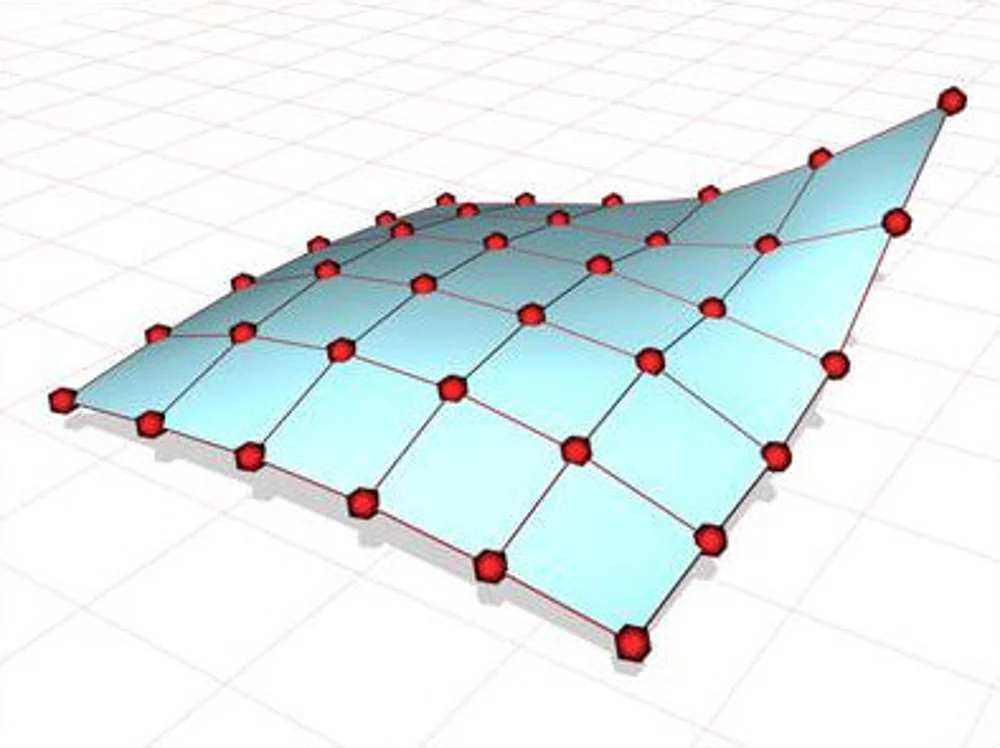
\includegraphics[max width=\linewidth]{slike/strukturePodatakaGeometrijaTehnika2.png}
			\caption{Прецизна мрежа}
			\label{fig:geomTehnika2}
		\end{minipage}
	\end{figure}

	\begin{figure}[H]
		\centering
		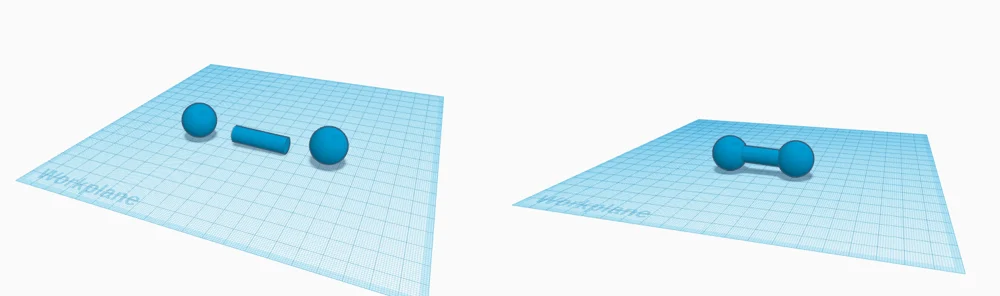
\includegraphics[max width=0.9\linewidth]{slike/strukturePodatakaGeometrijaTehnika3.png}
		\caption{Конструктивна геометрија чврстих тела}
		\label{fig:geomTehnika3}
	\end{figure}

	Што се тиче спољашњег изгледа, постоје два (најчешћа) начина како се они чувају:
	\begin{enumerate}
	\item Први начин би био мапирање текстуре. Овај начин је врло једноставан, и свака тачка на моделу се мапира на дводимензионалну слику (текстуру). Прво се мапирају темена модела на слику, а остале тачке интерполацијом добијају координате на слици (слика \ref{fig:izgledTehnika1}).
	\item Други начин би био да свакој страници доделимо неке особине које ће одредити како ће она изгледати (нпр. боја, текстура, материјал, итд) (слика \ref{fig:izgledTehnika2}).
	\end{enumerate}

	\begin{figure}[H]
		\begin{minipage}{0.4\linewidth}
			\centering
			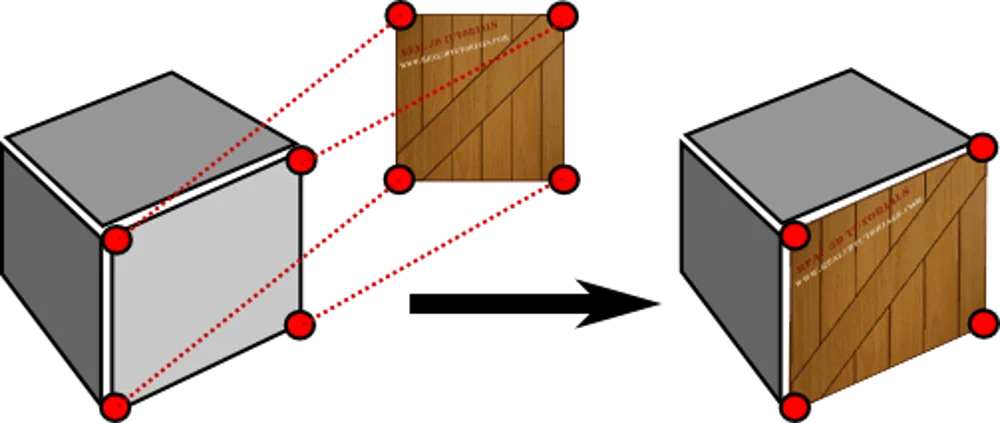
\includegraphics[max width=\linewidth]{slike/strukturePodatakaIzgledTehnika1.png}
			\caption{Мапирање текстуре}
			\label{fig:izgledTehnika1}
		\end{minipage}\hfill
		\begin{minipage}{0.4\linewidth}
			\centering
			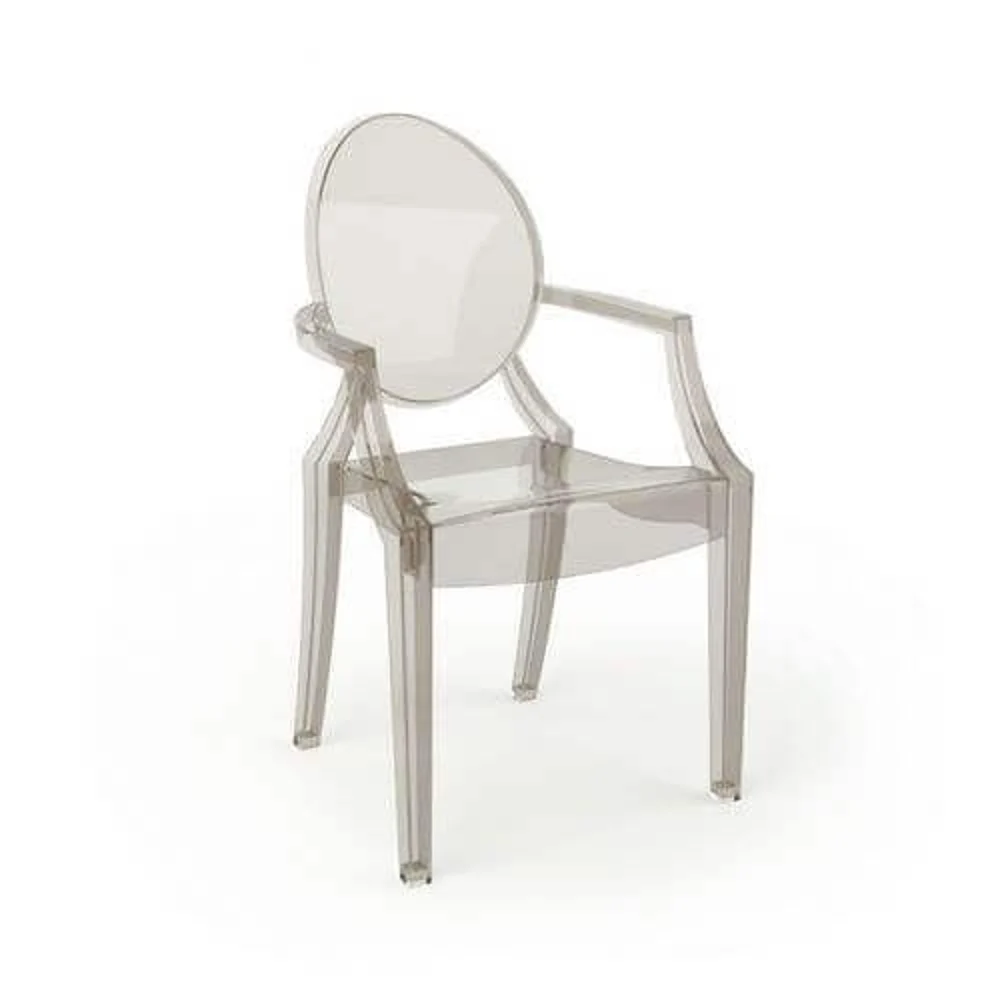
\includegraphics[max width=\linewidth]{slike/strukturePodatakaIzgledTehnika2.png}
			\caption{Странице са особинама}
			\label{fig:izgledTehnika2}
		\end{minipage}
	\end{figure}

	Морали бисмо споменути да модели нису једини могући објекти који су битни за рендеровање. Такође имамо објекте као што су камера и осветљење, који су неопходни за рендеровање. Камера представља наше гледиште из којег ћемо видети околину, односно из чијег гледишта ћемо рендеровати све. Камера садржи компоненте као што су позиција, смер ка коме је окренута, њен видокруг и вектор који је усмерен ка горе у односу на глобални координатни систем. Камера може бити перспективна или ортогонална. Што се тиче светла, постоји много различитих врста светлости (дирекционално, хелиоцентрично и још многе друге), и свака има своје компоненте. Најлакше би било описати тачкасту светлост која има само компоненте за позицију, боју и интентзитет.
	
	\subsection{Интерпретирање и процесуирање података}
	\paragraph{}
	Сада, када знамо каквим подацима баратамо, можемо да се упустимо у главни део, а то је како да ми те податке претворимо у слику коју можемо да прикажемо на екрану. Ово "како да ми те податке претворимо у слику" представљају различите технике рендеровања. Но, да не би дошло до забуне, на технике рендеровања више треба гледати као део целог процеса рендеровања, а не као нешто што га једнозначно дефинише, пошто у већини случајева ми ћемо користити више различитих техника како бисмо добили жељене резултате (као да ми те технике слажемо једне преко других). Из тог разлога бих технике рендеровања делио на више подгрупа, где свака подгрупа садржи различите фамилије техника који служе за добијање резултата које та подгрупа тражи. Прву велику подгрупу смо споменули, а то су технике које раде у реалном времену, и они који су спори. Друга велика подгрупа је сачињена од техника рендеровања које покушавају да добију видљиве информације сцене, односно визуелизација видљивих модела у нашем видокругу. У практичном смислу ми желимо да видимо шта наша камера у сцени види, и да то што она види можемо да нацртамо на екран. Фамилије техника ове подгрупе могли бисмо да сведемо на:
	\begin{enumerate}
	\item Z бафер - У овој фамилији техника, алгоритми функционишу по следећем принципу. Имамо један бафер који се зове z бафер и он чува z координату (дубину) која је најближа камери за сваки пиксел на екрану. Такође имамо бафер који се зове фрејм бафер и он чува податке о боји пиксела који се налазе у z баферу. Помоћу ова два бафера ми можемо да створимо слику коју ће монитор да нацрта, а између сваког фрејма ми ажурирамо наш z и фрејм бафер, како бисмо тачно нацртали оно што камера види.
	\item Скенирање линија - У ову фамилију техника спадају оне технике чији алгоритми функционишу по принципу да, за разлику од Z бафера који рачуна и чува пиксел по пиксел, он то ради ред по ред. За сваки ред (линију) пиксела на екрану, он чува странице модела које пресецају тај ред и сортира их од најближег левој страни до најдаљег левој страни (по x координати у растућем поретку). Ова структура се назива листа активних ивица. Проласком кроз ову листу ми добијамо информације о томе која површина је видљива за који пиксел у том реду.
	\item Испаљивање зракова - У овој фамилији техника, алгоритми функционишу тако што за сваки пиксел ми "испапалимо" један светлосни зрак из њега (односно из камере), и затим израчунамо у коју површину он прво удари, након чега гледамо да ли је могуће да из те тачке тај светлосни зрак доспе до извора светлости и у односу на исход овог процеса ми обојимо тај пиксел (у принципу, ми покушавамо да обрнемо процес доласка зрака до камере, односно нас). Алгоритми се могу разликовати по томе колико је дозвољено пута да се зрак одбије од површину, начин на који се рачуна тачка пресека зрака и објекта, начин на који се интерпретира резултат, итд. Описаћемо један алгоритам из ове фамилије - оцртавање сфера (страна \pageref{sfericnorenderovanje}).
	\item Оцртавање зракова - У ову фамилију техника спадају оне технике које, за разлику од испаљивања зракова где су путеви и понашања зракова више апроксимирани ради брзине, покушавају да у потпуности симулирају светлосне зраке. Из тог разлога алгоритми у овој фамилији стварају врло фотореалистичне слике, и тренутно је поље у компјутерској графици који се највише истражује. Данас је чак могуће да се ови алгоритми користе у реалном времену, али уз јако добар хардвер који то подржава (новије графичке картице чак имају јединице баш намењене за симулирање светлосних зракова).
	\end{enumerate}
	Као што сам рекао, обично се користи више различитих техника заједно како бисмо добили жељени резултат. Неке од фамилије техника које су такође битне, биле би технике које симулирају замагљеност при кретању, технике за анти-алијасинг (пошто пиксели нису бесконачно мали, неки детаљи који су мањи од величине пиксела нису могући да се виде, те може да се деси да слика коју добијемо буде пуна чудних и оштрих ивица; овај феномен се назива алијасинг, и можете га приметити када бисте отворили програм Паинт и нацртали косу линију), технике за одсјај сунца, итд.
	
	\subsection{Шејдери}
	\paragraph{}
	Прикупили смо податке, обрадили смо их и знамо тачно шта треба да се нацрта, односно како сваки пиксел треба да се обоји. Остало је још само (што се нас тиче) да пошаљемо те податке графичкој картици и да јој назначимо како шта треба да се нацрта, како би их она нацртала. Свака стандардна графичка картица има своје сетове инструкција које користи како би нацртала један фрејм (наравно постоје и графичке картице које је могуће да се програмирају од стране човека, али то нису графичке картице које се продају, односно које се користе, већ су специфично направљене због некакве потребе потрошача који је купује, те се њоме нећемо бавити), и ми морамо некако да јој кажемо како и шта она треба да нацрта, а сад како ће она то испод хаубе да уради, то је до ње. Стога, ми заправо користимо некакве оквире који су већ створени и помоћу драјвера ми "разговарамо" са графичком картицом. Ови оквири нам омогућавају да пошаљемо наше податке графичкој картици, а начин на који ми графичкој картици казујемо како да интерпретира и користи те податке јесте помоћу шејдера. Шејдери су у суштини програм, односно код који се извршава на графичкој картици. Они су прави програмски језици. У зависности од оквира који користимо, користићемо другачије програмске језике (нпр. OpenGL користи GLSL, док Direct3D користи Мајкрософтов HLSL). Чак иако су сви шејдери писани истим језиком унутар једног оквира, постоје различити шејдери у односу на њихову улогу, и они могу бити:
	\begin{enumerate}
	\item Фрагментни шејдери - ови шејдери ће бити извршени за сваки фрагмент, односно пиксел на екрану, и служе како би одредили боју и остале атрибуте фрагмента.
	\item Темени шејдери - ови шејдери ће бити извршени за свако теме које смо послали графичкој картици, и они претходе следећем кораку који је или геометријски шејдер (ако постоји), или растеризатор након чега долази на ред фрагментни шејдер.
	\item Геометријски шејдери - ови шејдери ће бити извршени за сваки примитивни објекат (тачке, линије, троуглови, итд), и служе како бисмо урадили нешто што бисмо иначе урадили за сваки примитивни објекат (нпр. стварање бачене сенке).
	\item Теселациони шејдери - ови шејдери нам служи за извршавање теселације, процес који смо споменули у одељку за структуре података (страна \pageref{strukturepodatakaproces}), што нам омогућава да по вољи добијемо већу резолуцију на моделима; Катмул-Кларков алгоритам (страна \pageref{katmulklark}) би био један од алгоритама који бисмо користили у теселационом шејдеру.
	\item Шејдери за оцртавање зракова - ови шејдери се користе при имплементирању техника из фамилије техника оцртавања зракова.
	\item Шејдери за рачунање - ови шејдери се користе за рачунање нечега, и чак се не морају користити само при рендеровању, већ се могу користити засебно ако нам је потребно да нешто извршавамо на графичкој картици (графичке картице су супериорније од процесора када нам је потребно да се изврши много једноставних паралелних операција).
	\end{enumerate}
	\paragraph{}
	Но, како бисмо све ово јасније и истинскије разумели, морали бисмо да ово ново знање употребимо практично. Направићемо апликацију у којој ћемо демонстрирати неке основне елементе целе досадашње приче.

	\pagebreak

	\section{Пример апликација у OpenGL-у}
	
	\subsection{Опис}
	\paragraph{}
	Направићемо врло једноставну апликацију у којој ћемо моћи да се помоћу тастатуре и миша крећемо око шарене коцке. Како бисмо комуницирали и сарађивали са графичком картицом, користићемо OpenGL. OpenGL сам по себи није никакав нити програм нити програмски језик, већ само спецификација која одређује како треба да једна његова имплементација изгледа, а саме имплементације стварају произвођачи графичких картица и можемо их пронаћи у драјверима графике картице. Разлози за коришћење OpenGL-а су то што је врло једноставан за коришћење (можете нацртати један троугао у само неколико редова пошто је много једноставнији од других; нпр. када бисмо користили  Vulkan, било би нам потребно абнормално више припреме како бисмо нацртали онај исти један троугао), функционише на свим оперативним системима, и одличан је за почетак и схватање основа. Пре но што  прионемо на саму логику коју ћемо имплементирати у коду, морамо видети каквим структурама података баратамо и разумети како оне функционишу. Пошто цртамо само обичну коцку, користићемо апроксимирану мрежу и све особине које одређују како ће коцка изгледати ћемо додељивати сваком троуглу у тој апроксимираној мрежи. Такође, коцку нећемо читати из никаквог фајла, већ ћемо ручно уписивати особине пошто коцка има само 8 темена.
	
	\subsection{Структуре података}
	
	\subsubsection{Бафери темена}
	\paragraph{}
	Структура бафер темена нам представља бафер (бафер је само некаква меморијска локација на коме се налазе подаци) у коме чувамо податке једне особине (позиција, боја, нормални вектор, итд) свих темена. Пошто је бафер темена заправо као један велики џак у коме се налази гомилу података, ми графичкој картици морамо да назначимо како да прочита податке који се налазе у баферу. Стога, ми уз бафер темена морамо доделити и његов атрибут, односно да му опишемо како су подаци чувани у њему (нпр. кажемо му да свако теме садржи по три цела броја, које ћемо после у шејдеру узимати и користити као координате позиције у три димензије). За сваку особину морамо имати по један бафер темена (у нашем случају потребни су нам два бафера темена, један за његову позицију, и један за његову боју).
	
	\subsubsection{Темени низ}
	\paragraph{}
	Структура темени низ нам представља објекат који нам служи како бисмо повезали бафере темена једне целине. Он не чува податке који се налазе унутар бафера темена, већ чува изглед и начин интерпретације бафера темена (његов атрибут) и локацију тог бафера темена. Користе се нпр. када имамо више различитих модела, па можемо једном, на почетку, да иницијализујемо бафере темена једног објекта унутар теменог низа, и када желимо поново да користимо тај објекат можемо користити његов темени низ.
	
	\subsubsection{Бафери индекса}
	\paragraph{}
	Структура бафер индекса нам представља бафер у којима чувамо индексе темена који сачињавају примитивне облике (најчешће је примитиван облик који цртамо троугао) тог модела. У случају троугла, ми у њему чувамо тројке целобројних вредности које представљају индексе темена објекта написане у смеру обрнутом од казаљке на сату, а особине тих темена смо проследили кроз бафере темена.
	
	\subsection{Процесуирање података}
	\paragraph{}
	Сада када имамо коцку записану у облику којим графичка картица може да рукује, пре него што кажемо графичкој картици да нацрта коцку морамо се позабавити са још једном ствари. Коцка коју смо описали је описана у односу на њен центар. Морамо да трансформишемо позиције њених темена из референтног система коцке, у референтни систем перспективе наше камере. Ово ћемо учинити помоћу математике, односно линеарне алгебре, но пошто је ово рад из области компјутерских наука, а не из области математике, нећу се удубљивати у тај рачун већ морате да ми верујете на реч да функционише.\footnote{Укратко речено, користићемо трансформације матрица како бисмо из једног референтног система прешли у други. Прво морамо из референтног система коцке да пређемо у референтни систем сцене, па из референтног система сцене у референтни систем камере. Ове две трансформације можемо постићи коришћењем матрица за транслирање. Последња трансформација јесте трансформација која ће трансформисати из ортогоналне пројекције у перспективу, и ову трансформацију ћемо постићи помоћу пројекционе матрице. Корисна особина матрица јесте да тиме што их множимо ми заправо чинимо једну трансформацију за другом, те можемо лакше да израчунамо свеукупну трансформацију ($P_{novo} = A\times B\times C\times P_{staro} = (A\times B\times C) \times P_{staro}$ значи да ће над позицијом прво бити извршена трансформација $C$, па онда трансформација $B$ и на крају трансформација $A$, и ради брзине ми можемо да $A\times B\times C$ израчунамо на процесору и добијену матрицу, као такву, пошаљемо графичкој картици). Та финално добијена матрица која садржи све три трансформације назива се енглеском MVP матрица (свако слово представља једну трансформацију).} Ове трансформације нећемо још извршити већ ћемо их само проследити графичкој картици као униформ (униформ представља променљиву коју можемо послати шејдеру), и која ће је извршити за нас (много је ефикасније пошто су графичке картице оптимизоване за матрични рачун,  и процесуирају све паралелно).  Остало је још само да одредимо и имплементирамо технику рендеровања. Користићемо Z бафер због његове једноставности и уместо да сами напишемо код за њега, можемо само да користимо имплементацију у драјверима која је након свих ових година (а Z бафер је једна од првих техника рендеровања) врло оптимизована, те добијамо и на брзини, а и на лакоћи "имплементирања". Тек сада можемо почети да цртамо нашу коцку. Графичкој сада треба да пошаљемо шејдере који ће јој назначити како да из тих података створи слику (већ смо рекли графичкој картици да користи технику Z бафер-а, али треба још и да изврши трансформацију позиција темена, и да обоји коцку помоћу боја које смо јој послали).
	
	\subsection{Шејдери}
	
	\subsubsection{GLSL}
	\paragraph{}
	OpenGL је створио програмски језик за шејдере под називом GLSL (енгл. GL Shading Language) и то је језик који ћемо користити за кодирање шејдера. GLSL по синтакси је копија C програмског језика, само што има уграђене функције и класе у себи које се често користе при рендеровању (нпр. имају уграђене матрице и векторе у себи, као и операције над њима, функције као минимум, максимум, апсолутна вредност вектора, итд), и нема неке функционалности које имају смисла само у програмима који се извршавају на процесору. Променљиве које шејдер прима су означене са in, док су променљиве које шејдер шаље следећем кораку у процесу означене су са out.
	
	\subsubsection{Темени шејдер}
	\paragraph{}
	  Све што ћемо урадити у овом шејдеру јесте да проследимо боју коју смо послали графичкој картици из процесора у следећи стадијум процеса (ништа не мењамо код боје), а над позицијом ћемо прво извршити трансформацију коју смо послали из процесора. Треба напоменути да све послате особине које нису позиција, као нпр. боја, ће бити интерполисане по површини троугла, односно, на примеру боје, свака тачка унутар троугла ће бити мешавина боја темена тог троугла, а у зависности од удаљености до темена, боја сваког темена ће бити мање или више присутна у произвољној тачки на троуглу. Код теменог шејдера:
	 \begin{lstlisting}[language=GLSL]
	 #version 330 core
	 
	 layout(location = 0) in vec3 pozicija;
	 layout(location = 1) in vec3 boja;
	 
	 out vec3 fBoja;
	 
	 uniform mat4 u_MVP;
	 
	 void main()
	 {	 
	 	fBoja = boja;
	 	gl_Position = u_MVP * vec4(pozicija, 1);
	 };
	 \end{lstlisting}
		
	\pagebreak
	
	\subsubsection{Фрагментни шејдер}
	\paragraph{}
	У фрагментном шејдеру нећемо радити ништа специјално, већ ћемо само проследити финалну боју пиксела како би се она нацртала. Код фрагментног шејдера:
	\begin{lstlisting}[language=GLSL]
	#version 330 core
	
	in vec3 fBoja;
	
	layout(location = 0) out vec4 boja;
	
	void main()
	{
		boja = vec4(fBoja, 1);
	};
	\end{lstlisting}
	
	\subsection{Резултат}
	\paragraph{}
	Након свега овог посла и кода који смо написали, можемо напокон да уберемо плодове нашег рада. Апликација функционише тако што мишем и тастатуром можемо да се крећемо око шарене коцке и да се дивимо њеној лепоти.
	
	\begin{figure}[H]
		\centering
		\begin{subfigure}{0.45\linewidth}
			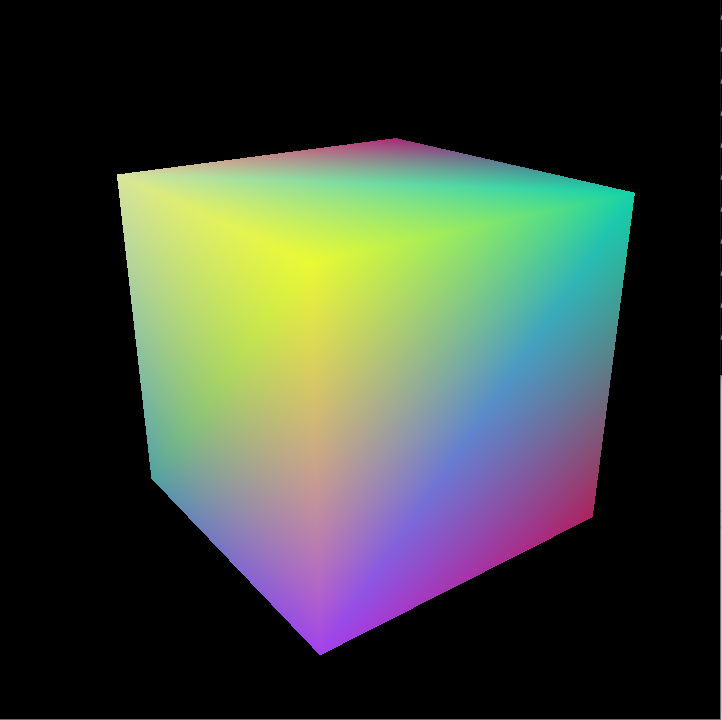
\includegraphics[width=\linewidth]{slike/aplikacijaSlika1.PNG}
		\end{subfigure}
		\begin{subfigure}{0.45\linewidth}
			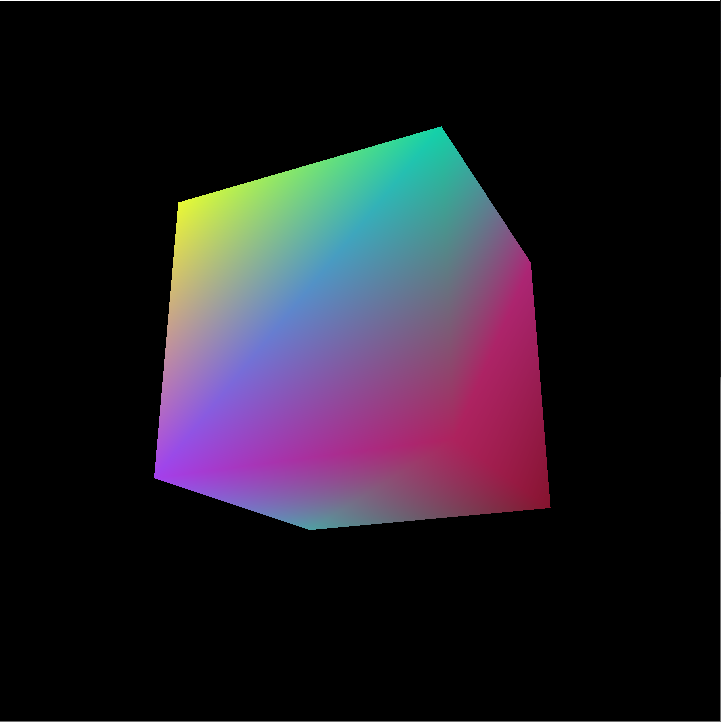
\includegraphics[width=\linewidth]{slike/aplikacijaSlika2.PNG}
		\end{subfigure}
		\caption{Слике апликације}
		\label{fig:katmulklark}
	\end{figure}
	
	\pagebreak
	
	\section{Технике рендеровања}
	
	\subsection{Оцртавање сфера}\label{sfericnorenderovanje}
	\paragraph{}
	Овај алгоритам функционише, као што на основном нивоу функционишу и остали алгоритми ове фамилије техника, тако што за сваки пиксел на екрану испали по један зрак. "Испаљивање" се извршава тако што се прво израчуна најближа тачка у односу на тренутну позицију зрака и затим се зрак помери у напред за ту дужину. Овакав начин померања нам омогућава да са сигурношћу зрак никада не прође кроз неки објекат. Овај процес понављамо док зрак или не додирне неки објекат, или не пређе пут који је већи од удаљености коју смо ми одредили, те само одредимо да се није ни са чим сударио и нацртамо само боју неба за тај пиксел (слика \ref{fig:ocrtavanjezrakova}). Ако се деси судар зрака са објектом, имамо две могућности: да очитамо вредност боје објекта и у односу на то да ли се и под којим углом сунце види ту тачку нацртамо боју пиксела, или да одбијемо зрак у нормалном правцу у односну на објекат у тој тачки. Ове одбитке можемо извршавати колико ми пута желимо, и сваки одбитак нам даје информације које можемо користити како бисмо израчунали крајњу боју пиксела.
	\paragraph{}
	Овај алгоритам нам такође омогућава да добијемо још неке ефекте као споредни производ. На пример, можемо јако лако детектовати ивице тако што ако удаљеност најближе тачке буде јако близу (ми одређујемо колико је јако близу заправо близу променљивом) оној удаљености за коју кажемо да је дошло до судара, али у том тренутку крене да се удаљеност повећава, то мора значити да смо детектовали ивицу објекта (слика \ref{fig:detekcijaIvice}).
	\paragraph{}
	Најтежи део имплементације овог алгоритма јесте кодирање функције која одређује удаљеност зрака од објеката, и од зависности њене имплементације зависи и брзина кода. Постоје разне оптимизације, од тога које објекте (па самим тим и тачке) узимамо као могуће кандидате (нпр. К-Д дрво), до тога на који начин рачунамо удаљености до објеката (не морамо користити еуклидску геометрију).  Најзанимљивији део овог алгоритма и јесте то што све ове оптимизације и начини имплементације истог алгоритма могу прозивести резултате који се толико разликују једни од других, те тиме што се мало поиграте у коду можете видети разне занимљиве исходе (слика \ref{fig:fraktali}).
	
	\begin{figure}[H]
		\centering
		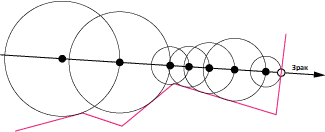
\includegraphics[max width=0.45\linewidth]{slike/ocrtavanjeZrakova.png}
		\caption{Пример једног циклуса путовања зрака}
		\label{fig:ocrtavanjezrakova}
	\end{figure}
	
	\begin{figure}[H]
		\begin{minipage}{0.4\linewidth}
			\centering
			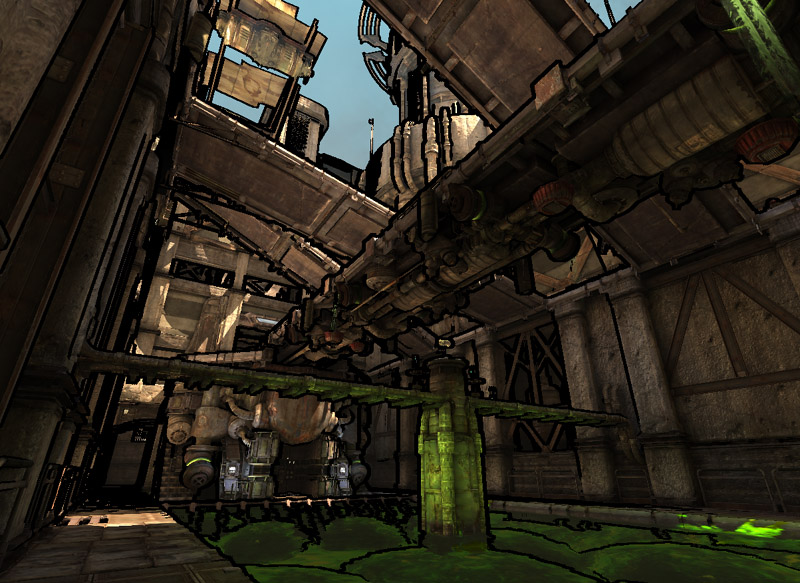
\includegraphics[max width=\linewidth]{slike/primerDetekcijeIvice.jpg}
			\caption{Слика добијена тако што када детектујемо ивицу нацртамо црн пиксел}
			\label{fig:detekcijaIvice}
		\end{minipage}\hfill
		\begin{minipage}{0.5\linewidth}
			\centering
			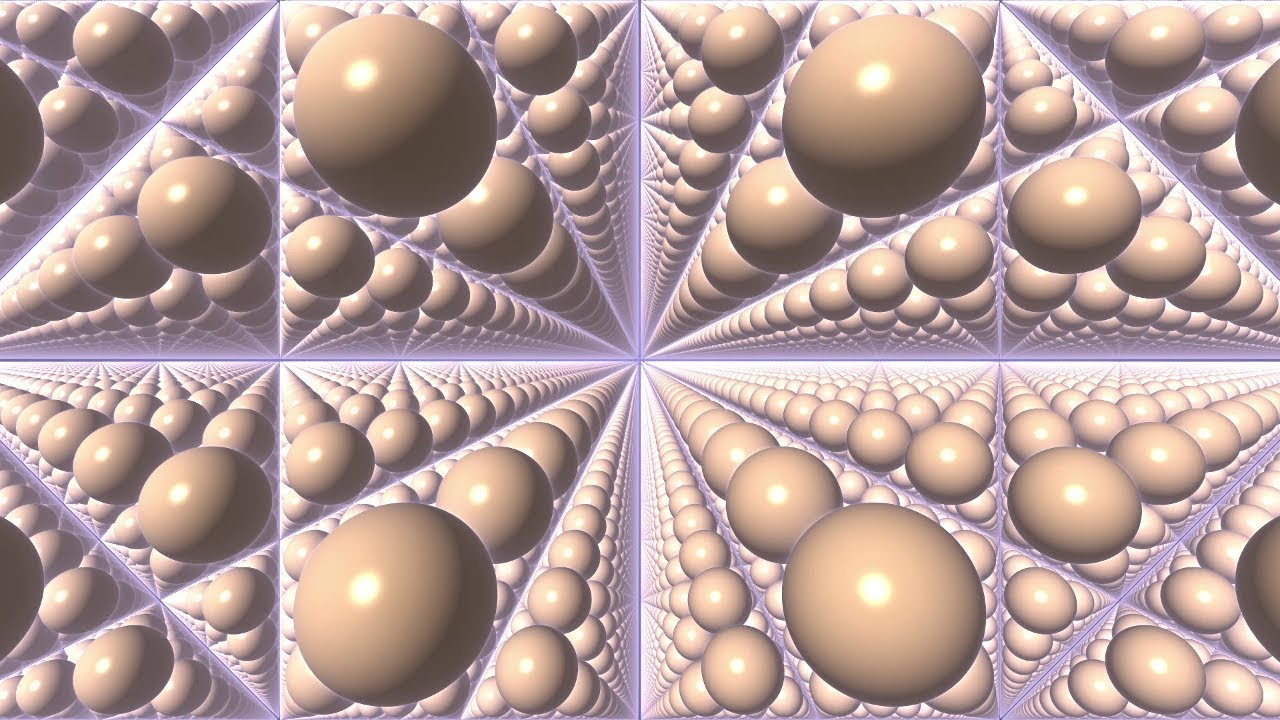
\includegraphics[max width=\linewidth]{slike/kdDrvoFraktali.jpg}
			\caption{Фрактал добијен чудноватијом имплементацијом К-Д дрвета}
			\label{fig:fraktali}
		\end{minipage}
	\end{figure}
	
	\subsection{Разни алгоритми везани за рендеровање}
	
	\subsubsection{Коен-Сатерландов алгоритам}\label{koensaterland}
	\paragraph{}
	Алгоритам жели да подели екран (гледамо као да је он дводимензионална раван) на 9 једнаких региона и одреди које линије или делови линија припадају средишњем региону. Алгоритам се изводи следећим корацима:
	\begin{enumerate}
		\item Свакој крајњој тачки се припоји код региона. Код региона је четворобитни број који означава у којем се региону налази тачка, први бит је 1 ако се тачка налази изнад средишњег региона, други бит је 1 ако се тачка налази испод средишњег региона, трећи бит је 1 ако се тачка налази десно од средишњег региона, четврти бит је 1 ако се тачка налази лево од средишњег региона.
		\item Линија у целости припада региону ако обе крајње тачке имају код региона 0000.
		\item У супротном, логичка (битска) и операција се врши између кодова региона крајњих тачака.
		\begin{enumerate}
			\item[3.1.] Ако резултат није 0000, линија у целости не припада средишњем региону.
			\item[3.2.] У супротном, морамо да одсечемо део који не припада средишњем региону.
			\begin{enumerate}
				\item[3.2.1.] Изаберемо крајњу тачку линије која не припада средишњем региону.
				\item[3.2.2.] Пронађемо тачку пресека линије са ивицама средишњим регионом која је најближа изабраној крајњој тачки.
				\item[3.2.3.] Изабрану крајњу тачку заменимо са тачком пресека.
				\item[3.2.4.] Поновити корак 2.
			\end{enumerate}
		\end{enumerate}
	\end{enumerate}
	
	\subsubsection{Катмул-Кларков алгоритам}\label{katmulklark}
	\paragraph{}
	Алгоритам жели да дода темена телу тако да се добије облије тело у односу на почетно тело. Пошто овај алгоритам ради на било којем конвексном телу, процес можемо извршити жељени број пута за редом, односно можемо је користити рекурзивно толико пута колико нам је потребно да бисмо добили жељени степен облине.  Алгоритам се изводи следећим корацима:
	\begin{enumerate}
		\item За сваку страну додајемо по једну тачку стране, чију позицију добијамо тиме што узмемо средњу вредност позиција темена које чине ту страну (слика \ref{fig:katmulklark}a).
		\item За сваку ивицу додајемо по једну тачку ивице, чију позицију добијамо тиме што узмемо средњу вредност позиција темена које чине ту ивицу (слика \ref{fig:katmulklark}b).
		\item За свако оригинално теме ($P$) израчунамо средњу вредност ($F$) свих $n$ (које смо мало пре створили) темена страница где страница додирује тачку $P$ и израчунамо средњу вредност ($R$) свих $n$ средишта ивица оригиналних ивица које додирују тачку $P$, где је свако средиште ивица једнако средњој вредности позиција крајева те ивице (слика \ref{fig:katmulklark}c).
		\begin{align}
			P_{novo}&=\frac{F+2R+(n-3)P}{n}
		\end{align}
		
		\item Формирати ивице и стране нове мреже.
		\begin{enumerate}
			\item[4.1.] Повезати сваку нову тачку стране са новим тачкама ивице које припадају оригиналној ивици која је сачињавала оригиналну страну (слика \ref{fig:katmulklark}d).
			\item[4.2.] Повезати нова темена са новим тачкама ивице које припадају оригиналној ивици која је садржала оригинално теме (слика \ref{fig:katmulklark}e).
			\item[4.3.] Оформите нове стране које су затворене новим ивицама (слика \ref{fig:katmulklark}f).
		\end{enumerate}
	\end{enumerate}


	\begin{figure}[H]
		\centering
		\begin{subfigure}{0.3\linewidth}
			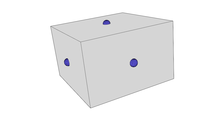
\includegraphics[width=\linewidth]{slike/Catmull-Clark_Recursive_Step_1.png}
			\caption{Тачке стране (плаве сфере)}
		\end{subfigure}
		\begin{subfigure}{0.3\linewidth}
			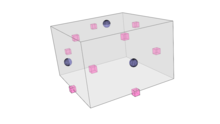
\includegraphics[width=\linewidth]{slike/Catmull-Clark_Recursive_Step_2.png}
			\caption{Тачке ивице (розе коцке)}
		\end{subfigure}
		\begin{subfigure}{0.3\linewidth}
			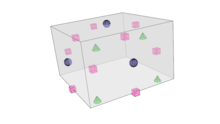
\includegraphics[width=\linewidth]{slike/Catmull-Clark_Recursive_Step_3.png}
			\caption{Нова темена (зелене купе)}
		\end{subfigure}
		\begin{subfigure}{0.3\linewidth}
			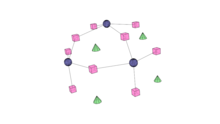
\includegraphics[width=\linewidth]{slike/Catmull-Clark_Recursive_Step_4.png}
			\caption{Нове ивице, четири по тачки стране}
		\end{subfigure}
		\begin{subfigure}{0.3\linewidth}
			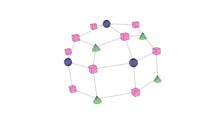
\includegraphics[width=\linewidth]{slike/Catmull-Clark_Recursive_Step_5.png}
			\caption{Три нове ивице по новом темену}
		\end{subfigure}
		\begin{subfigure}{0.3\linewidth}
			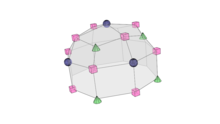
\includegraphics[width=\linewidth]{slike/Catmull-Clark_Recursive_Step_6.png}
			\caption{Завршно додавање страна на мрежу}
		\end{subfigure}
		\caption{Илустрација корака Катмул-Кларковог алгоритма}
		\label{fig:katmulklark}
	\end{figure}

	\pagebreak

	\section{Референце}
	https://en.wikipedia.org/wiki/Computer\_graphics\_(computer\_science)\\
	https://www.graphics.cornell.edu/about/what-computer-graphics\\
	https://www.techopedia.com/definition/9163/rendering\\
	https://firstrender.net/\\
	https://en.wikipedia.org/wiki/University\_of\_Utah\_School\_of\_Computing\\
	https://pixelperfect-studios.com/history-of-3d-rendering/\\
	https://medium.com/@antoinefortin\_64750/the-little-history-of-rendering-1-3a7f30cb633\\
	https://en.wikipedia.org/wiki/Cohen\%E2\%80\%93Sutherland\_algorithm\\
	https://en.wikipedia.org/wiki/Catmull\%E2\%80\%93Clark\_subdivision\_surface\\
	https://www.youtube.com/watch?v=OyotbIxO-UQ\&ab\_channel=Education4u\\
	https://all3dp.com/3d-file-format-3d-files-3d-printer-3d-cad-vrml-stl-obj/\\
	https://biblus.accasoftware.com/en/rendering-definition-types-and-visualization-techniques/\\
	https://en.wikipedia.org/wiki/Rendering\_(computer\_graphics)\\
	https://www.javatpoint.com/computer-graphics-z-buffer-algorithm\\
	https://www.javatpoint.com/computer-graphics-scan-line-algorithm\\
	https://www.youtube.com/channel/UCQ-W1KE9EYfdxhL6S4twUNw\\
	https://en.wikipedia.org/wiki/Shader\\
	https://stackoverflow.com/questions/25570116/difference-between-tessellation-shaders-and-geometry-shaders\\
	https://www.youtube.com/watch?v=Cp5WWtMoeKg\&ab\_channel=SebastianLague\\
	https://www.youtube.com/watch?v=svLzmFuSBhk\&ab\_channel=CodeParade\\
	
\end{document}